% !TEX encoding = UTF-8 Unicode
\documentclass[11pt]{exam}
\usepackage{amsmath}
\usepackage{amssymb}
\usepackage{enumerate}
\usepackage{dsfont}
\usepackage[utf8x]{inputenc}
\usepackage{booktabs}
\usepackage[usenames,dvipsnames]{xcolor}
\usepackage[dutch]{babel}
\usepackage{multi	col}
\usepackage{tikz}

%\renewcommand*\rmdefault{iwona}
%\usepackage[math]{iwona}
%\usepackage[math]{kurier}


%Evenwijdig symbool
\newcommand{\nevenwijdig}{\,\rlap{$\diagdown$} /\hspace{-0.2em}/\,}
\newcommand{\evenwijdig}{\,/\hspace{-0.2em}/\,}

% New definition of square root:
% it renames \sqrt as \oldsqrt
\let\oldsqrt\sqrt
% it defines the new \sqrt in terms of the old one
\def\sqrt{\mathpalette\DHLhksqrt}
\def\DHLhksqrt#1#2{\setbox0=\hbox{$#1\oldsqrt{#2\,}$}\dimen0=\ht0
\advance\dimen0-0.2\ht0
\setbox2=\hbox{\vrule height\ht0 depth -\dimen0}%
{\box0\lower0.4pt\box2}}

\printanswers
\addpoints
\shadedsolutions 
\definecolor{HeadColor}{rgb}{0.65,0.65,0.65}
\definecolor{SolutionColor}{rgb}{0.95,0.95,0.95}
\renewcommand{\solutiontitle}{\noindent\textbf{Oplossing:}\par\noindent}
\renewcommand\thepartno{\alph{partno}}
\renewcommand\partlabel{(\thepartno)} 

\renewcommand\questionlabel{\thesection.\thequestion}

\newcommand*{\QED}{\hfill\ensuremath{\square}}%
\newcommand*{\QEF}{\hfill\ensuremath{\diamond}}%
\author{Nathan Carter}
\title{Visual Group Theory}

\setlength{\parindent}{0pt}

%HEADER & FOOTEr
\pagestyle{empty} 

\begin{document}
\maketitle
\thispagestyle{empty}


\section{What is a group?}
\begin{questions}
	\question Group?
	
	\question Group?
	
	\question Group?
	
	\question Three walls in your bedroom hold pieces of art, one hung on each wall. You are rearranging them to see which arrangement best suits your taste. You cannot use the fourth wall, because it has a window.
	\begin{parts}
		\part Count the number of ways there are to rearrange the pictures, as long as only one is hung on each wall.
		\begin{solution}
			There are 6 possible configurations.
		\end{solution}
		
		\part Consider two actions: You may swap the art on the left wall with the art on the center wall, and you may swap the art on the center wall with the art on the right wall. Can these actions alone generate all of the configurations you counted?
		\begin{solution}
			\par Yes, consider
			\[ abc \rightarrow bac \rightarrow bca\rightarrow cba \rightarrow cab\rightarrow acb\]
		\end{solution}
		
		\part Does part (b) describe a group? If not, waht rule or rules were broken?
		\begin{solution}
			\par It describes a group.
		\end{solution}

	\end{parts}

\end{questions}
 %What is a group?
\section{What do groups look like?}
\begin{questions}
	\question In the rectangle puzzle, what actions were the generators? What other actions are there besides the generators?
	\begin{solution}
		\par Horizontal flip and vertical flip
		\par Other actions are the `do nothing' and the `horizontal followed by the vertical flip'
	\end{solution}
	
	\question In the light switch puzzle, what actions were the generators? What other actions are there besides the generators?
	\begin{solution}
		\par See previous exercice
	\end{solution}
	
	\question Can an arrow in a Cayley diagrem ever connect a node to itself?
	\begin{solution}
		\par Yes, the `do nothing' action.
	\end{solution}

	\question Exercices 1.1 of Chapter 1 defined a group. Create its Cayley diagram using the technique from this chapter.
	\begin{solution}
		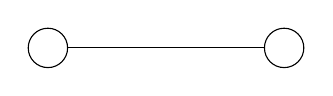
\begin{tikzpicture}
			\draw (0,0) -- (3,0);
			\draw[fill=white] (3,0) circle (0.25cm);
			\draw[fill=white] (0,0) circle (0.25cm);
		\end{tikzpicture}
	\end{solution}
	
	\question Exercise 1.4 of Chapter 1 defined a group. Create its Cayley diagram using the technique from this chapter.
	\begin{solution}
		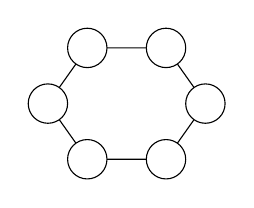
\begin{tikzpicture}
			\draw (0.5,0.707) -- (1,0) -- (0.5,-0.707) -- (-0.5,-0.707) -- (-1,0) -- (-0.5,0.707) --cycle;
			\draw[fill=white] (1,0) circle (0.25cm);
			\draw[fill=white] (0.5,0.707) circle (0.25cm);
			\draw[fill=white] (0.5,-0.707) circle (0.25cm);
			\draw[fill=white] (-0.5,0.707) circle (0.25cm);
			\draw[fill=white] (-0.5,-0.707) circle (0.25cm);
			\draw[fill=white] (-1,0) circle (0.25cm);
		\end{tikzpicture}
	\end{solution}

	\question Exercise 1.13 describes an infinite group which can be generated with just one generator. Can you draw an infinite Cayley diagram for it? (Just draw a portion of the diagram that makes the infinite pattern clear)
	\par How does that Cayley diagram compare to one for the group in Exercise 1.14 part (a)?
	
	\question Exercise 1.14 part (d) described a two-element group. Can you draw a Cayley diagram for it? Which arrow or arrows should you use and why?
	\begin{solution}
		\par $1 \leftrightarrow -1$ en op beide element een pijl naar zichzelf voor de actie `$\cdot 1$'.
	\end{solution}

	\question Section 2.2 introduced the rectangle puzzle. Imagine instead a square puzzle with its corners labeled the same way. Such a puzzle would allow a new move that was not possible with the rectangle puzzle, you could rotate a quarter-turn clockwise.
	\begin{parts}
		\part Make the map of this group
		\begin{solution}
			Zie $D_4$
		\end{solution}

		\part Why is the quarter-turn move not `allowed' in the rectangle puzzle?
		\begin{solution}
			Zie later
		\end{solution}
	\end{parts}
	
	\question Most groups can be generated may different ways, and each way gives rise to a corresponding way to connect a Cayley diagram with arrows. For example, consider the group $V_4$, which we met in the rectangle puzzle. Let's shorten the names of its actions to $n, h, v$ and $b$, meaning (respectively) no action, horizontal flip, vertical flip, and both (a horizontal flip followed by a vertical flip).
	\par We sam that $h$ and $v$ together generate $V_4$. But it is also true that $h$ and $b$ together would generate $V_4$, or $v$ an $b$ together. (You can verify these facts by exploring the rectangle realm using these generators on your own numbered rectangle.)
	\begin{parts}
		\part Make a copy of Figure 2.9 and add to it a new type of arrow, representing the action $b$.
		\begin{solution}
			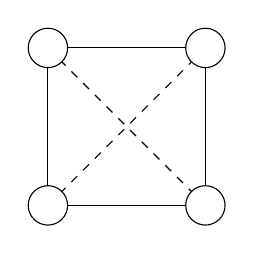
\begin{tikzpicture}
				\draw (0,0) -- (2,0) -- (2,2) -- (0,2) -- cycle;
				\draw[dashed] (0,0) -- (2,2);
				\draw[dashed] (0,2) -- (2,0);
				\draw[fill=white] (0,0) circle (0.25cm);
				\draw[fill=white] (0,2) circle (0.25cm);
				\draw[fill=white] (2,2) circle (0.25cm);
				\draw[fill=white] (2,0) circle (0.25cm);
			\end{tikzpicture}
		\end{solution}

		\part Make a copy of your answer  to part (a), with the arrows representing $h$ removed. How does your diagram show that $v$ and $b$ are sufficient to generate $V_4$?
		\begin{solution}
			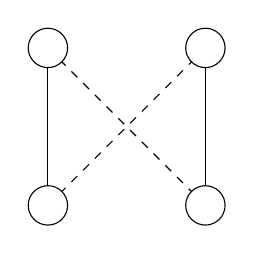
\begin{tikzpicture}
				\draw (2,0) -- (2,2);
				\draw (0,0) -- (0,2);
				\draw[dashed] (0,0) -- (2,2);
				\draw[dashed] (0,2) -- (2,0);
				\draw[fill=white] (0,0) circle (0.25cm);
				\draw[fill=white] (0,2) circle (0.25cm);
				\draw[fill=white] (2,2) circle (0.25cm);
				\draw[fill=white] (2,0) circle (0.25cm);
			\end{tikzpicture}
			\par It is still possible to reach each situation.
		\end{solution}
		
		\part Make a copy of your answer to part (a)n, with the arrows representing $v$ removed. How does your diagram show that $h$ and $b$ are sufficient to generate $V_4$?
		\begin{solution}
			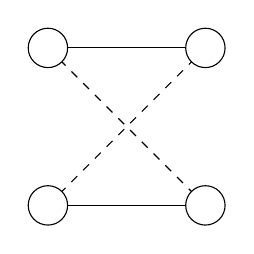
\begin{tikzpicture}
				\draw (0,0) -- (2,0);
				\draw (0,2) -- (2,2);
				\draw[dashed] (0,0) -- (2,2);
				\draw[dashed] (0,2) -- (2,0);
				\draw[fill=white] (0,0) circle (0.25cm);
				\draw[fill=white] (0,2) circle (0.25cm);
				\draw[fill=white] (2,2) circle (0.25cm);
				\draw[fill=white] (2,0) circle (0.25cm);
			\end{tikzpicture}
			\par It is still possible to reach each situation.
		\end{solution}
	\end{parts}

	\question If you've done all the exercises to this point, you've encountered two different Cayley diagrams that have the two-node form shown here.
	\par Can you come up with another group whose Cayley diagram has this form?
	
	\question If you've done all the exercices to this point, you've encountered two different Cayley diagrams that have the four-node form shown here.
	\par Can you come up with another group whose Cayley diagram has this form?
	
	\question We have not yet seen a group whose Cayley diagram has the three-node form called $C_3$, shown in the top left of Figure 2.10. Can you come up with a group whose Cayley diagram has that form?
	
	\question A group's generators have a special status in a Cayley diagram for the group. What is that special status?
	\begin{solution}
		Represented by the arrows.
	\end{solution}
	
	\question Chapter 1 required groups to satisfy Rule 1.5, which states, ``There is a predefined list of actions that never changes.'' How does this rule impact the appearance of Cayley diagrams? (Or how would diagrams be different if this rule were not a requirement?)
	\begin{solution}
		If a action would not be executed on a certain node.
	\end{solution}
	
	\question Chapter 1 required groups to satisfy Rule 1.6, which states, ``Every action is reversible.'' What constraint does this place on the arrows in a Cayley diagram? Can you draw a diagram that does not fit this constraint? (That is, draw a diagram that almost deservers the name ``Cayley diagram'', except for that one rule violation.)
	\begin{solution}
		Every node should have an arrow departing and arriving.
	\end{solution}

	\question Chapter 1 required groups to satisfy Rule 1.7, which states, ``Every action is deterministic.'' What constraint does this place on the arrows in a Cayley diagram? Can you draw a diagram that does not fit this constraint? (That is, draw a diagram that almost deserves the name ``Cayley diagram,'' except for that one rule violation.)
	\begin{solution}
		An arrow departing from a node can only arrive in one node.
	\end{solution}
	
	\question Chapter 1 required groups to satisfy Rule 1.8, which states, ``Any sequence of consecutive actions is also an action.'' How do we depend upon this fact when using a Cayley diagram as a map?
	\begin{solution}
		One should be able to reach every node by executing consecutive actions.
	\end{solution}
	
	\question If we created a equilateral triangle puzzle, like the square puzzle in exercise 2.8, what would the valid moves be? Map the group of such a puzzle.
	\begin{solution}
		\par Flip with respect to any symmetry axis. (Three flips) And a rotation over 60\textdegree, 120\textdegree and 180\textdegree. 
		\par This forms $D_3$.
		\par It has 2 generating actions, one flip and one rotation.
	\end{solution}

	\question A regular $n$-gon is a polygon with $n$ equal sieds an $n$ equal angles. You have already analyzed regular $n$-gons with $n=3$. (equilateral triangle, Exercise 2.18) and $n=4$ (square, Exercise 2.18).
	\begin{parts}
		\part Based on what you know about the cases $n=3$ and $n=3$, make a conjecture about how many actions will be in the group of a regular $n$-gon for any $n>2$.
		\begin{solution}
			There are $n$ axes of symmetry and $n$ rotations of 360\textdegree$:n$. This results in $2n$ symmetries.
		\end{solution}
		
		\part Test your conjecture by making te map of the group for a regular pentagon ($n=5$).
		\begin{solution}
			$D_5$ has 10 symmetries.
		\end{solution}
	\end{parts}
\end{questions} %What do groups look like?
\section{Why study groups?} %Why study groups?
\section{Algebra at last}
\begin{questions}
	\question Consider the lightswitch group shown in Figure 2.8. Let $L$ stand for the action of flipping the left switch and $R$ stand for the action of flipping the right switch.
	\begin{parts}
		\part Which of the following equations are true and which are false in this group?
		\begin{solution}
			\par $LRRRR = RRL$
			\par $LR=RLRLRL$
			\par $L\not = RR$
			\par $R^8 = R^{100}$
		\end{solution}

		\part Let $N$ stand for the non-action (leaving the switches untouched). Which of the following equations are true?
		\begin{solution}
			\par $(LNR)^2 \not = LNR$
			\par $RL \not = N$
			\par $(LNR)^3 = R^3L^3$
			\par $NN = N$
			\par $R^4 = N$
			\par $LRLR = N$
		\end{solution}
		
		\part What is the smallest power or $R$ that equals $N$?
		\begin{solution}
			\par $2$
		\end{solution}

		\part What is the smallest power or $L$ that equals $N$?
		\begin{solution}
			\par $2$
		\end{solution}

		\part What is the smallest power or $RL$ that equals $N$?
		\begin{solution}
			\par $2$
		\end{solution}

		\part What is the smallest power or $LR$ that equals $N$?
		\begin{solution}
			\par $2$
		\end{solution}
	\end{parts}
	
	\question 
	\begin{parts}
		\part Apply the transformations in Definition 4.1 to the lightswitch Cayley diagram in Figure 2.8.
		
		\part Create a multiplication table for the lightswitch group
		\begin{solution}
			\[
				\begin{array}{|c|c|c|c|}
				\hline
				e & L & R & LR\\
				\hline
				L & e & LR & R\\
				\hline
				R & LR & e & L\\
				\hline
				LR & R & L & e\\
				\hline
				\end{array}
			\]
		\end{solution}
	\end{parts}

	\question Each part below describes a set with a binary operation on it. For each one, determine whether it is commutative and whether it is associative.
	\begin{parts}
		\part the addition operation on the set of all whole numbers
		\begin{solution}
			\par commutative and associative
		\end{solution}

		\part the subtraction operation on the set of all whole numbers
		\begin{solution}
			\par not commutative and not associative
		\end{solution}
		
		\part the multiplication operation on the set of positive real numbers
		\begin{solution}
			\par commutative and associative
		\end{solution}

		\part the division operation on the set of positive real numbers
		\begin{solution}
			\par not commutative and not associative
		\end{solution}
		
		\part the exponentiation operation on the set of positive whole numbers (that is, the operation written $a^b$)
		\begin{solution}
			\par not commutative and not associative
		\end{solution}
	\end{parts}

	\question The Cayley diagrams for two groups are shown here, the cyclic group $C_5$ on the left and the Quaternion group $Q_4$ on the right.
	\begin{parts}
		\part The red arrow in the diagram for $C_5$ represents multiplication wby what element?
		\begin{solution}
			\par $\cdot a$
		\end{solution}
		
		\part What is $a^3 \cdot a$ in $C_5$?
		\begin{solution}
			\par $a^4$
		\end{solution}
		
		\part What is $a^3 \cdot a\cdot a$ in $C_5$?
		\begin{solution}
			\par $e$
		\end{solution}
		
		\part If $1$ is the identity element, then wat do red arrows in the diagram for $Q_4$ represent? What do blue arrows represent?
		\begin{solution}
			\par red $= \cdot i$
			\par blue $= \cdot j$
		\end{solution}
		
		\part What is $i^2$? What is $j\cdot i$?
		\begin{solution}
			\par $i^2 = -1$, $j\cdot i = k$
		\end{solution}
		
		\part What is $i\cdot j\cdot j$?
		\begin{solution}
			\par $-i$
		\end{solution}
	\end{parts}
	
	\question Using the Cayley diagrams from Exercise 4.4, answer the following questions.
	\begin{parts}
		\part How do you use the diagram of $C_5$ to multiply $x\cdot a^2$ in $C_5$, for any element $x$?
		\begin{solution}
			\par Rotate two turns.
		\end{solution}
		
		\part How do you use the diagram of $Q_4$ to multiply $x\cdot k$ in $Q_4$, for any element $x$?
		\begin{solution}
			\par Notice how $k = j\cdot i$, then $\cdot k$ means one has to follow a blue arrow, and then a red arrow.
		\end{solution}
	\end{parts}
	
	\question Create a multiplication table for each of the following Cayley diagrams.
	\begin{parts}
		\part $C_5$, as shown on the left of Exercise 4.4. Use the template given here.
		\begin{solution}
			\[
				\begin{array}{|c|c|c|c|c|}
				\hline
				e & a & a^2 & a^3 & a^4\\
				\hline
				a & a^2 & a^3 & a^4 & e\\
				\hline
				a^2 & a^3 & a^4 & e & a\\
				\hline
				a^3 & a^4 & e & a & a^2\\
				\hline
				a^4 & e & a & a^2 & a^3\\
				\hline
				\end{array}
			\]
		\end{solution}
		
		\part $Q_4$, the quaternion group with eight elements, as shown on the right of Exercise 4.5. Use the template given here.
		\begin{solution}
			\[
				\begin{array}{|c|c|c|c|c|c|c|c|}
				\hline
				1 & i & j & k & -1 & -i & -j & -k\\
				\hline
				i & -1 & k & -j & -i & 1 & -k & j\\
				\hline
				j & -k & -1 & i & -j & k & 1 & -i\\
				\hline
				k & j & -i & -1 & -k & -j & i & 1\\
				\hline
				-1 & -i & -j & -k & 1 & i & j & k\\
				\hline
				-i & 1 & -k & j & i & -1 & k & -j\\
				\hline
				-j & k & 1 & -i & j & -k & -1 & i\\
				\hline
				-k & -j & i & 1 & k & j & -i & -1\\
				\hline
				\end{array}
			\]
		\end{solution}

		\part $A_4$, the alternating group with twelve elements:
		\begin{solution}
			\[
				\begin{array}{|c|c|c|c|c|c|c|c|c|c|c|c|}
				\hline
				e & a & b & c & d & a^2 & b^2 & c^2 & d^2 & x & y & z\\
				\hline
				a & a^2 & c^2 & d^2 & b^2 & e & y & x & z & b & d & c\\
				\hline
				b & d^2 & b^2 & a^2 & c^2 & y & e & z & x & a & c & d\\
				\hline
				c & b^2 & d^2 & c^2 & a^2 &x & z & e & y & d & b & a\\
				\hline
				d & c^2 & a^2 & b^2 & d^2 & z & x & y & e & c & a & b\\
				\hline
				a^2 & e & x & z & y & a & d & b & c & c^2 & b^2 & d^2\\
				\hline 
				b^2 & x & e & y & z & c & b & d & a & d^2 & a^2 & c^2\\
				\hline
				c^2 & z & y & e & x & d & a & c & b & a^2 & d^2 & b^2\\
				\hline
				d^2 & y & z & x & e & b & c & a & d & b^2 & c^2 & a^2\\
				\hline
				x & c & d & a & b & b^2 & a^2 & d^2 & c^2 & e & z & y\\
				\hline
				y & b & a & d & c & d^2 & c^2 & b^2 & a^2 & z & e & x\\
				\hline
				z & d & c & b & a & c^2 & d^2 & a^2 & b^2 & y & x & e\\
				\hline
				\end{array}
			\]
		\end{solution}
	\end{parts}

	\question It is possible to suggest the full multiplication table for an infinite group by showing just part of it. Fill in the following partial table for the operation of addition on the set of all whole numbers; the ellipses indicate the table continues infinitely in all directions.

	\question Exercises 2.4 through 2.8 of Chapter 2 asked you to draw Cayley diagrams for three groups. Use the diagrams you drew to make multiplication tables for those same groups. Note that if your diagram is not yet a diagram of actions, you may need to apply the transformation in Definition 4.1.
	
	\question Exercises 2.18 and 2.19 of Chapter 2 asked you to find the pattern describing the sequence of Cayley diagrams for the ``n-gon puzzle.'' I mentioned in that exercise that the family of groups describing such puzzles are called the dihedral groups. You will study them in detail in Chapter 5, and this exercise previews some of that material.
	\par Find the pattern decsribing the sequence of multiplication tables for those same groups. You might consider the following steps.
	\begin{parts}
		\part Create multiplication tables from the Cayley diagrams for triangle, square, and regular pentagon puzzles.
		\begin{solution}
			\par Triangle
			\[
				\begin{array}{|c|c|c|c|c|c|}
				\hline
				e & r & r^2 & f & rf & r^2f\\
				\hline
				r & r^2 & e & rf & r^2f & f\\
				\hline
				r^2 & e & r & r^2f & f & rf\\
				\hline 
				f & r^2f & rf & e & r^2 & r\\
				\hline
				rf & f & r^2f & r & e & r^2\\
				\hline
				r^2f & rf & f & r^2 & r & e\\
				\hline
				\end{array}
			\]
			
			\par Square
			\[
				\begin{array}{|c|c|c|c|c|c|c|c|}
				\hline
				e & r & r^2 & r^3 & f & rf & r^2f & r^3f\\
				\hline
				r & r^2 & r^3 & e & rf & r^2f & r^3f & f\\
				\hline
				r^2 & r^3 & e & r & r^2f & r^3f & f & rf\\
				\hline
				r^3 & e & r & r^2 & r^3f & f & rf & r^2f\\
				\hline 
				f & r^3f & r^2f & rf & e & r^3 & r^2 & r\\
				\hline
				rf & f & r^3f & r^2f & r & e & r^3 & r^2\\
				\hline
				r^2f & rf & f & r^3f & r^2 & r & e & r^3\\
				\hline
				r^3f & r^2f & rf & f & r^3 & r^2 & r & e\\
				\hline
				\end{array}
			\]
			\par Notice how smaller squares can be found in the large square. The Cayley-graph has an inner and outer circle. 
		\end{solution}
	\end{parts}

	\question Consider te following multiplication table that displays an binary operation.
	\begin{parts}
		\part Explain succinctly why the binary operation is not associative. Can you write your answer as one equation?
		\begin{solution}
			\par Consider $A\cdot A\cdot B$, then $A\cdot (A\cdot B) = A\cdot e = A$ while $(A\cdot A)\cdot B = e \cdot B = B$
		\end{solution}
		
		\part Does the operation have inverses?
		\begin{solution}
			\par Yes, but they are not unique. (See also Exercise 4.11)
		\end{solution}
	\end{parts}

	\question Consider the following multiplication table that displays a binary operation.
	\begin{parts}
		\part Explain succinctly why the binary operation does not have inverses. Can you write your answers as one equation?
		\begin{solution}
			\par Notice how $3$ is the identity element. But notice how there is no inverse for $2$ and inverse for $1$.
		\end{solution}
		
		\part Is the operation associative?
		\begin{solution}
			\par Yes.
		\end{solution}
	\end{parts}

	\question Consider the following multiplication table that displays a binary operation.
	\begin{parts}
		\part Does this operation have inverses? Justify your answer.
		\begin{solution}
			\par No, $x$ and $y$ have no inverses.
		\end{solution}

		\part Is the operation associative? Justify your answer.
		\begin{solution}
			\par Seems like it.
		\end{solution}
	\end{parts}
	
	\question For each multiplication table below, explain why it does not depict a group.
	\begin{parts}
		\part Not associative, $(4\cdot 2)\cdot 3 = 1\cdot 3 = 3$ while $4\cdot (2\cdot 3) = 4\cdot e = 4$.
		\part $a,b,c$ have no inverses.
		\part Not associative, $(c\cdot a)\cdot c = c\cdot c = e$ while $c\cdot (a\cdot c) = c\cdot a = c$.
		\part There is no identity.
	\end{parts}
	
	\question The following multiplication table does not depict a binary operation on the set $\{e,x,y\}$. The reason is part of the definition of a binary operation; we would say that this binary operation lacks \textbf{closure}. Can you spot the problem and explain it in your own words?
	\begin{solution}
		\par $y\cdot x = s\not \in \{ e,x,y\}$.
	\end{solution}

	\question Why can the same element not appear twice in any row of a group's multiplication table? Does this restriction also apply to columns?
	\begin{solution}
		\par If $a\cdot b = a\cdot c$ then $b=c$, since $a^{-1}\cdot a\cdot b = c \Rightarrow b = c$.
		\par The same rule applies for columns. $a\cdot b = c\cdot b \Rightarrow a=c$.
	\end{solution}

	\question Exercises \ldots
	
	\question When crating a multiplication table for a group, if you try to include two different identity elements, what goes wrong? What does this lead you to conclude about groups?
	\begin{solution}
		\par Then the multiplication table will have the same element appearing twice in a row and column. Because $e\cdot b = \tilde e\cdot b \Rightarrow e=\tilde e$.
	\end{solution}

	\question Explain why a Cayley diagram must be connected. That is, why must there be a path from every node to every node?
	\begin{solution}
		\par If this is not the case, then some element will appear twice in a row or column.
		\par Different motivation, the identity element would not be connected to everything.
	\end{solution}
	
	\question Complete each of the following multiplication tables so that it depicts a group. There is only one way to do so, if we require $0$ to be the identity element in each table. Then search Group Explorer's group librrary to determine the names for the groups the tables represent.
	\begin{solution}
		\begin{parts}
			\part $C_2$
			\[
				\begin{array}{|c|c|}
					\hline
					0 & 1\\
					\hline
					1 & 0\\
					\hline
				\end{array}
			\]
			
			\part $C_3$
			\[
				\begin{array}{|c|c|c|}
					\hline
					0 & 1 & 2\\
					\hline
					1 & 2 & 0\\
					\hline
					2 & 0 & 1\\
					\hline
				\end{array}
			\]
			
			\part $C_1 = \{ 0\}$
			\[
				\begin{array}{|c|}
					\hline
					0 \\
					\hline
				\end{array}
			\]
			
			\part $C_4$
			\[
				\begin{array}{|c|c|c|c|}
					\hline
					0 & 1 & 2 & 3\\
					\hline
					1 & 2 & 3 & 0\\
					\hline
					2 & 3 & 0 & 1\\
					\hline
					3 & 0 & 1 & 2\\
					\hline
				\end{array}
			\]
			
			\part Looks like $V_4$?
			\[
				\begin{array}{|c|c|c|c|}
					\hline
					0 & 1 & 2 & 3\\
					\hline
					1 & 3 & 0 & 2\\
					\hline
					2 & 0 & 3 & 1\\
					\hline
					3 & 2 & 1 & 0\\
					\hline
				\end{array}
			\]
		\end{parts}
	\end{solution}

	\question The following table can be completed in more than one way, and still have the result depict a group. Find all possible such completions of the table, again using $0$ as the identity element. How many did you find? Search Group Explorer's group library to determine the names for the groups each of your resulting tables represents.
	
	
	\question From Exercise 4.19 part (a) you can conclude that there is only one pattern for a group containing two elements. This is because the only difference between the multiplication table you computed and that of any other group with two elements will be the names of those elements. So the pattern of interactions among elements (or colors if we were to color the cells of the table) would be no different.
	\begin{parts}
		\part How many patterns are there for groups containing three elements?
		\begin{solution}
			\par Only one, $C_3$.
		\end{solution}

		\part Containing one elements?
		\begin{solution}
			\par Only one, $\{e\} = 1$.
		\end{solution}
		
		\part Containing four elements?
		\begin{solution}
			\par Two, $V_4$ and $C_4$.
		\end{solution}
	\end{parts}
	
	\question We saw earlier in this chapter that in the group $V_4$, the equation $RB=BR$ is true. In fact, for any two elements $a,b\in V_4$, the equation $ab=ba$ is true. That is, the order in which you combine elements does not matter. Consider each group whose multiplication table appears in Figure 4.7 (except $A_5$, whose details are to small to see). For which of those groups does the order of combining elements matter?
	\begin{solution}
		\par $S_3$, Quasihedral group with 16 elements.
	\end{solution}

	\question Groups in which he order of multiplication of elements does not matter are called commutative or abelian. Look through the groups in Group Explorer's group library, starting with the smallest, until you find one that is noncommutative. What is the name of the smallest noncummutative group?
	\begin{solution}
		$S_3$ of order 6.
	\end{solution}

	\question What visual pattern do the multiplication tables of commutative groups exhibit?
 	\begin{solution}
		\par Diagonal symmetry.
	\end{solution}

	\question To go along with the other algebraic notation we've seen in this chapter, there is also an algebraic notation for generators. For instance, the group $C_5$, which appears in the first few exercises of this chapter, is generated by the element $a$. The standard notation for this is $C_5 = \langle a\rangle$. The $\langle a\rangle$ means ``what you can generate from $a$,'' and so the equation $C_5=\langle a\rangle$ is saying ``$C_5$ is the group generated from $a$.'' From Figure 4.3, we can write $V_4 = \langle R,B\rangle$, saying that $R$ and $B$ together generate $V_4$.
	\par Show your understanding of this new notation by filling in the blanks below using however many elements are necessary to generate the group. Use as few elements as possible.
	\begin{parts}
		\part From the Cayley diagram in Exercise 4.4, we see that $Q_4 =\langle _ \rangle $
		\begin{solution}
			$Q_4 = \langle i, j\rangle$
		\end{solution}

		\part From the Cayley diagram in part (c) of Exercise 4.6, we see that $A_4 =\langle _ \rangle $
		\begin{solution}
			$A_4 = \langle a, x \rangle$
		\end{solution}
	\end{parts}
	
	\question Use the multiplication tables you constructed in Exercise 4.6 to determine the inverses for each element of each of the three groups from that problem.
	\begin{parts}
		\part In the cyclic group $C_5$, the inverses are
		\begin{solution}
			\par $e^{-1} = e, a^{-1} = a^4, (a^{2})^{-1} = a^{3}, \ldots$
		\end{solution}

		\part In the quaternion group $Q_4$, the inverses are
		\begin{solution}
			\par $1^{-1} = 1, i^{-1} = -i, j^{-1} = -j, k^{-1}=-k$
			\par $(-1)^{-1} = -1, (-i)^{-1} = i, \ldots$
		\end{solution}
		
		\part In the alternating group $A_4$, the inverses are
		\begin{solution}
			\par $e^{-1} = e, a^{-1} = a^2, b^{-1} = b^2, c^{-1} = c^2, \ldots$
		\end{solution}
	\end{parts}

	\question Inverses can be used to solve equations. In the group $C_5$, to solve $a^2x=a$ for $x$, I can proceed as in high school algebra:
	\par Computing $(a^2)^{-1} a$ in $C_5$ gives $x=a^4$.
	\par Try solving each of these equation in $C_5$.
	\begin{parts}
		\part $a^3x = a^2$
		\begin{solution}
			\par $\Leftrightarrow x= a^4$
		\end{solution}

		\part $a^4a^2x = a$
		\begin{solution}
			\par $\Leftrightarrow ax = a$
			\par $\Leftrightarrow x = e$
		\end{solution}

		\part $ax(a^3)^{-1} = e$
		\begin{solution}
			\par $\Leftrightarrow ax = a^3$
			\par $\Leftrightarrow x = a^2$
		\end{solution}
	\end{parts}

	\question 
	\begin{parts}
		\part If I have the equation $a^2x(a^2)^{-1} = a$ to solve as in the previous exercise, can I cancel the $a^2$ and the $(a^2)^{-1}$? Why or why not?
		\begin{solution}
			\par Yes, as $C_5$ is abelian.
		\end{solution}

		\part If I have a similar equation, but in the group $Q_4$ from Exercise 4.6, $ixi^{-1} = j$, can I cancel the $i$ and $i^{-1}$? Why or why not?
		\begin{solution}
			\par No, as it is not abelian. 
			\par Note how $i\cdot j \cdot i^{-1} = k\cdot (-i) = -j \not = j$
		\end{solution}
	\end{parts}

	\question Consider the equation $b^2\cdot t\cdot a^2 = y$ in the group $A_4$; I want to solve for $t$. The previous exercise as ia warning that I cannot simply proceed as follows. What should I do instead?
	\begin{solution}
		\par $\Leftrightarrow t\cdot a^2 = (b^2)^{-1}\cdot y = b\cdot y = c$
		\par $\Leftrightarrow t = c\cdot (a^2)^{-1} = c\cdot a = b^2$
	\end{solution}

	\question Solve these equations for $t$.
	\begin{parts}
		\part In $Q_4, jitk^{-1} = -kj$
		\begin{solution}
			\par $\Leftrightarrow -kt = i\cdot k$
			\par $\Leftrightarrow t = (-k)^{-1} \cdot (-j)$
			\par $\Leftrightarrow t = k\cdot(-j) = i$
		\end{solution}

		\part In $A_4, t(b^2)^2 = xyz$
		\begin{solution}
			\par $\Leftrightarrow t b = e$
			\par $\Leftrightarrow t = b^{-1} = b^2$
		\end{solution}

		\part In $S_3, rtf = e$
		\begin{solution}
			\par $\Leftrightarrow rt = f$
			\par $\Leftrightarrow t = r^2\cdot f = fr$
		\end{solution}
	\end{parts}

	\question Let's say you have a group $G$ with identity element $e$. Take any three elements $a,b,$ and $c$ in $G$.
	\begin{parts}
		\part What does the equation $ab=e$ say about the relationship between $a$ and $b$?
		\begin{solution}
			\par $a$ is the inverse of $b$ and vice versa.
		\end{solution}

		\part If both $ab=e$ and $ac = e$, can you use algebra to show $b=c$?
		\begin{solution}
			\par It follows that $ab=ac \Rightarrow b = a^{-1}ac = c$.
		\end{solution}
		
		\part Can an element in a group have two different inverses?
		\begin{solution}
			\par No, since $a^{-1} \cdot a = \tilde{a^{-1}} a \Rightarrow a^{-1} = \tilde{a^{-1}}$.
		\end{solution}
	\end{parts}

	\question The set of all integers (all positive and negative whole numbers, and zero) is often written als $\mathds{Z}$. Use Definition 4.2 to answer each of the following questions about $\mathds{Z}$.
	\begin{parts}
		\part Is it a group using ordinary addition as the operation?
		\begin{solution}
			\par Yes.
		\end{solution}

		\part Is it a group using ordinary multiplication as the operation?
		\begin{solution}
			\par No, there are inverses missing.
		\end{solution}
		
		\part The even integers are sometimes written $2\mathds{Z}$, because they can be obtained by multiplying every integer by 2. If we think of $3\mathds{Z}, 4\mathds{Z}$, and in general any $n\mathds{Z}$ in the same way, for what integers $n$ is the set $n\mathds{Z}$ a group using ordinary addition as the operation?
		\begin{solution}
			\par $\forall n\in \mathds{Z}$.
		\end{solution}
	\end{parts}

	\question The rational numbers (often written $\mathds{Q}$) are the set of fractions $\frac{a}{b}$, where $a$ and $b$ are integers (but $b\not = 0$). For example $\frac{1}{2}, \frac{-6}{11},$ and $\frac{50}{3}$ are all rational. Any integer, including zero, is rational, because you can just divide it by 1. For example, 10 is the rational number $\frac{10}{1}$.
	\par Use Definition 4.2 to answer each of the following question about $\mathds{Q}$.
	\begin{parts}
		\part Is it a group using ordinary addition as the operation?
		\begin{solution}
			\par Yes.
		\end{solution}
		
		\part Is it a group using ordinary multiplication as the operation?
		\begin{solution}
			\par No, zero has no inverse.
		\end{solution}
		
		\part Call $\mathds{Q}^+$ the positive rational numbers (only those greater than zero). Is $\mathds{Q}^+$ a group using ordinary addition as the operation?
		\begin{solution}
			\par No, there is no identity and no inverses.
		\end{solution}

		\part Is $\mathds{Q}^+$ a group under ordinary multiplication?
		\begin{solution}
			\par Yes.
		\end{solution}
		
		\part Call $\mathds{Q}^*$ the nonzero rational numbers (all positive and negative ones, only leaving out zero). Is $\mathds{Q}^*$ a group under ordinary addition?
		\begin{solution}
			\par No, there is no identity.
		\end{solution}

		\part Is $\mathds{Q}^*$ a group under ordinary multiplication?
		\begin{solution}
			\par Yes.
		\end{solution}
		
		\part Why are groups like $\mathds{Q}, \mathds{Q}^+,$ and $\mathds{Q}^*$ difficult to visualize using multiplication tables and Cayley diagrams?
		\begin{solution}
			\par Because they are difficult to list\ldots
		\end{solution}
	\end{parts}
\end{questions} %Algebra at last
\section{Five families}
\begin{questions}
	\question If a group is generated by just one elemnt, what kind of group is it?
	\begin{solution}
		A cyclic group
	\end{solution}

	\question
	\begin{parts}
		\part In the group $C_5$, compute $2+2$.
		\begin{solution}
			\par $2+2 = 4$
		\end{solution}

		\part In the group $C_5$, compute $4+3$.
		\begin{solution}
			\par $4+3 = 2$
		\end{solution}
		
		\part In the group $C_{10}$, compute $8+7$.
		\begin{solution}
			\par $8+7 =5$
		\end{solution}
		
		\part In the group $C_{10}$, compute $9+1$.
		\begin{solution}
			\par $9+1 = 0$
		\end{solution}
		
		\part In the group $C_3$, compute $2+2+2+2+2+2$.
		\begin{solution}
			\par $2+2+2+2+2+2 = 0$
		\end{solution}
		
		\part In the group $C_{11}$, compute $10-8+1-7+6+5$.
		\begin{solution}
			\par $10-8+1-7+6+5 = -4 = 7$
		\end{solution}
	\end{parts}

	\question For each statement below, determine if it is true or false.
	\begin{parts}
		\part Every cyclic group is abelian.
		\begin{solution}
			\par True.
		\end{solution}

		\part Ever abelian group is cyclic.
		\begin{solution}
			\par False, consider $V_4$
		\end{solution}
		
		\part Every dihedral group is abelian.
		\begin{solution}
			\par False, consider $D_4$, then $\sigma \circ \tau_X \not = \tau_X \circ \sigma$.
		\end{solution}
		
		\part Some cyclic groups are dihedral.
		\begin{solution}
			\par False, it would imply that some dihedral groups are abelian. Which is false.
		\end{solution}
		
		\part There is a cyclic group of order 100.
		\begin{solution}
			\par True, $C_{100}$.
		\end{solution}

		\part There is a symmetric group of order 100.
		\begin{solution}
			\par False, $|S_4| = 4! = 24$ while $|S_5| = 5! = 120$
		\end{solution}
		
		\part If some pair of elements in a group commute, the group is abelian.
		\begin{solution}
			\par False, consider $D_4$.
		\end{solution}
		
		\part If every pair of elements in a group commute, the group is cyclic.
		\begin{solution}
			\par False, consider $V_4$.
		\end{solution}
		
		\part If the pattern on the left of Figure 5.8 appears nowhere in the Cayley diagram for a group, then the group is abelian.
		\begin{solution}
			\par True.
		\end{solution}
	\end{parts}
	
	\question
	\begin{parts}
		\part Use the Cayley diagram of the group $D_5$ in Figure 5.17 to compute $r\cdot f\cdot r$ in that group.
		\begin{solution}
			$r\cdot f \cdot r =f$
		\end{solution}

		\part Is the answer the same or different if you do the computation in the group $D_3$ instead?
		\begin{solution}
			$r\cdot f \cdot r =f$
		\end{solution}
		
		\part Is the answer the same or different if you do the computation in the group $D_n$ instead?
		\begin{solution}
			\par $r\cdot f \cdot r = f$, because $r\cdot f = r^{-1} \cdot ? = f\cdot r \cdot f \cdot ?$, which results in $? = f^{-1}=f$.
		\end{solution}
	\end{parts}

	\question Compare the strengths and weaknesses of the tree visualization techniques introduced in this book: Cayley diagrams, multiplication tables, and cycle graphs.
	
	\question Sketch the following visualizations.
	\begin{parts}
		\part a cycle graph for $C_9$
		\part a Cayley diagram for $D_4$
		\part a multiplication table for $D_2$
		\begin{solution}
			\[
				\begin{array}{|c|c|}
					\hline
					0 & 1 \\
					\hline
					1 & 0 \\
					\hline
				\end{array}
			\]
		\end{solution}
	\end{parts}

	\question Describe in words what each of the following visualizations look like for $C_{999}$
	\begin{parts}
		\part Cayley diagram
		\part multiplication table
		\part cycle graph
	\end{parts}

	\question Describe in words what each of the following visualizations look like for $D_{999}$
	\begin{parts}
		\part Cayley diagram
		\part multiplication table
		\part cycle graph
	\end{parts}
	
	\question What are the orders for the first ten symmetric groups, $S_1$ through $S_{10}$? What are the orders of their corresponding alternating groups, $A_1$ trough $A_{10}$? Explain your answer for the order of $A_1$.
	\begin{solution}
		\par $|S_n| = n!$
		
		\par Since $A_1$ is constructed by considering the squares of elements from $S_1$ one counts $|A_1| = 1$.
		
		\par $|A_2| = 1$ while $|S_2| = 2$,
		\par $|A_3| = 3$ (Figure 5.25) while $|S_3| = 3! = 6$
		\par $|A_4| = 12$
		\par $|A_n| = n! : 2$
	\end{solution}

	\question The exercises for Chapter 3 asked you to create several Cayley diagrams. This chapter introduced a mehtod for telling whether a group is abelian based on its Cayley diagram. For each of the Chapter 3 exercises mentioned below, first determine whether the group belongs to any of the five families introduced in this chapter, and if so, what the group's name is (e.g. $D_4, S_3,$ etc.). Explain how you determine each of your answers.


	\question Explain why every cyclic group is abelian.
	\begin{solution}
		\par Rotations around a fixed center is a commutative operation.
	\end{solution}
	
	\question Qhy is it sufficient, when looking to see if a Cayley diagram represents an abelian group, to only consider the arrows? Why do we not need to examine every possible combination of paths?
	\begin{solution}
		\par Because the path is a constructed as a sequence of arrows.
	\end{solution}
	
	\question 
	\begin{parts}
		\part Create a cycle graph for the group $V_4$ using the multiplication table in Figure 5.31.
		\begin{solution}
			petal flower with three petals
		\end{solution}

		\part Create a cycle graph for the group $A_4$ using the Cayley diagram in Exercise 4.6 part (c).
		\begin{solution}
			Four 2 node petals, 3 1 node petal
		\end{solution}
	\end{parts}

	\question
	\begin{parts}
		\part Is there a dihedral group of order 7?
		\begin{solution}
			\par No $|D_n| = 2n$
		\end{solution}

		\part If $A_n$ has order $2520$, what is $n$?
		\begin{solution}
			\par $7, 7! = 5040$
		\end{solution}

		\part If $A_n$ has order $m$, what order does $S_n$ have?
		\begin{solution}
			$2m$
		\end{solution}
	\end{parts}

	\question For each part below, compute the orbit of the element in the group. Your answer will be alist of elements from the group that ends with the identity.
	\begin{parts}
		\part The element $r^2$ in the group $D_{10}$
		\begin{solution}
			\par $= \{ r^2, r^4, r^6, r^8, e\}$
		\end{solution}

		\part The element $10$ in the group $C_{16}$
		\begin{solution}
			\par $= \{ 10, 4, 14, 8, 2, 12, 6, 0\}$
		\end{solution}

		\part The element $25$ in the group $C_{30}$
		\begin{solution}
			\par $= \{25, 20, 15, 10, 5, 0 \}$
		\end{solution}

		\part The element $12$ in the group $C_{42}$
		\begin{solution}
			\par $=\{12, 24, 36, 6, 18, 30, 0 \}$
		\end{solution}

		\part The element $s$ in the group whose Cayley diagram is on the left below. (Assume the element $a$ at the top left is the identity.)
		\begin{solution}
			\par $=\{ s, m, j, a\}$
		\end{solution}

		\part The element $l$ in the group whose Cayley diagram is on the right below. (Assume the element $a$ at the top is the identity.)
		\begin{solution}
			\par $=\{ l, e, p, a\}$
		\end{solution}
	\end{parts}

	\question Recall the notation for generators from Exercise 4.25. Use it to fill in the blanks below with however many elements necessary to generate the group. Use as few elements as possible.
	\begin{parts}
		\part $C_n= \{0,1,\ldots, n-1\}$
		\begin{solution}
			\par $= \langle 1\rangle$
		\end{solution}
		
		\part $D_n=\{ e,r,\ldots r^{n-1}, f,fr,\ldots, fr^{n-1}\}$
		\begin{solution}
			\par $= \langle r,f\rangle$
		\end{solution}
	\end{parts}
	
	\question Create multiplication tables for the smallest dihedral groups $D_1, D_2, D_3$ and so on, until you find the first non-abelian member of the family. Which is it an how can you tell?
	\begin{solution}
		\par $D_1$
		\[
			\begin{array}{|c|}
			\hline
			e\\
			\hline
			\end{array}
		\]
		\par $D_2$
		\[
			\begin{array}{|c|c|}
			\hline
			e& r\\
			\hline
			r & e\\
			\hline
			\end{array}
		\]
		\par $D_3$
		\[
			\begin{array}{|c|c|c|c|c|c|}
			\hline
			e & r & r^2 & f & rf & r^2f\\
			\hline
			r & r^2 & e & rf & r^2 f & f\\
			\hline
			r^2 & e & r & r^2f & f & rf\\
			\hline
			f & r^2f & rf & e & r^2 & r\\
			\hline
			rf & f & r^2f & r & e & r^2\\
			\hline
			r^2f & rf & f & r^2 & r & e\\
			\hline 
			\end{array}
		\]
		\par Is niet Abels. Zo geldt bijvoorbeeld dat $fr = r^2f$ terwijl $rf = rf$.
	\end{solution}
	
	\question Repeat Exercise 5.17 for the symmetric groups $S_n$. Use the permutation notation from this chapter.
	\begin{solution}
		\par $S_1$
		\[
			\begin{array}{|c|}
			\hline
			e\\
			\hline
			\end{array}
		\]
		\par $S_2$
		\[
			\begin{array}{|c|c|}
			\hline
			e& (1 2)\\
			\hline
			(1 2) & e\\
			\hline
			\end{array}
		\]
		\par $S_3$
		\[
			\begin{array}{|c|c|c|c|c|c|}
			\hline
			e& (1 2)(3) & (1)(2 3) & (1 3)(2) & (1 2 3) & (1 3 2)\\
			\hline
			(1 2)(3) & e & (123) & (132) & (1)(23)&(13)(2) \\
			\hline
			(1)(23) & (132) & e & (123) & (13)(2) & (12)(3)\\
			\hline
			(13)(2) & (123) & (132) & e & (12)(3) & (1)(23)\\
			\hline
			(123) & (13)(2) & (12)(3) & (1)(23) & (132) & e\\
			\hline
			(132) & (1)(23) & (13)(2) & (12)(3) & e & (123)\\
			\hline
			\end{array}
		\]
		\par Is niet Abels.
	\end{solution}

	\question For each symmetric group whose multiplication table you created in Exercise 5.18, compute the elements of the corresponding alternating group, as in Figure 5.25. For each alternating group you compute, create
	\begin{parts}
		\part a multiplication table,
		\begin{solution}
			\par $A_1 = S_1$
			\par $A_2 = S_1$
			\par $A_3 = \{ e, (123), (132)\}$
			\[
				\begin{array}{|c|c|c|}
				\hline
				e& (1 2 3) & (132)\\
				\hline
				(123) & (132) & e\\
				\hline
				(132) & e & (123)\\
				\hline
				\end{array}
			\]
		\end{solution}

		\part a Cayley diagram, and
		\part a cycle graph
	\end{parts}

	\question Some of the smallest meembers of the families $C_n,D_n, S_n$ and $A_n$ actually belong to more than one family, as long as we do not care about the names of the elements, but about the group structure. For instance, $D_1$ is a group with two elements, and its mulitplicationt able has the same pattern as that of $C_2$, as shown here.
	\par What other groups belong to more than one of the families we studied in this chapter? (Another way to read this question is, ``are there any groups of the families $C_n, D_n, S_n,$ or $A_n$ that are isomorphic to a group in another of those families?'')
	
	\begin{solution}
		\par $D_1\cong S_1\cong C_1 \cong A_1$
		\par $D_2\cong S_2 \cong C_2$
		\par $C_3\cong A_3$
		\par $D_3\cong S_3$
	\end{solution}

	\question For each of the following questions, either exhibit a group that answers the question in the affirmative or give a clear explanation of thy the answer to the question is negative.
	\begin{parts}
		\part Is here a cyclic group with exactly four generators? (Not that it takes four elements to generate the group, but that there are four different elements $a,b,c,d$ in $C_n$ and $C_n = \langle a\rangle =\langle b\rangle =\langle c\rangle \langle d\rangle.$) Is there more than one such group?
		\begin{solution}
			\par Yes, $C_8$ with generators $\{ 1,3,5,7\}$
			\par $C_5$ with generators $\{1,2,3,4 \}$ complies as well.
		\end{solution}
	
		\part Is there a cyclic group with exactly one generator? Is there more than one?
		\begin{solution}
			\par Both $C_1 = \langle 0\rangle$ and $C_2=\langle 1\rangle$ comply.
		\end{solution}
	\end{parts}
	
	\question Group Explorer
	
	\question Broad
	
	\question This chapter gave regular polygons as examples of objects whose symmetries are described by dihedral groups, that is, objects with both rotational and bilateral symmetry, but no other symmetries. What other objects fit in this category?
	\begin{solution}
		\par Snowflakes, rounded polygons, \ldots
	\end{solution}
	
	\question Analyze the symmetries of a tetrahedro using the technique from Defintion 3.1, resulting in the Cayley diagram for its symmetry group. Here are a few hints to get you started.
	
	\question As you now from this chapter, $S_3$ and $D_3$ are two different names for the same group. Yet no larger dihedral group is also a symmetric group. Give an argument based on the physical featers of a $n$-gon for why this is so? $(n\geqslant 4)$.
	\begin{solution}
		\par $n! \geqslant 2n$ when $n\geqslant 4$. A regular $n$-gon has exactly $n$ axis of symmetry, and $n$ rotations resulting in $2n$ transformations.
	\end{solution}
	
	\question Section 5.2.3 describes what the cycle graph will look like for $C_p\times C_p$ if $p$ is a prime number. Draw the cycle graph for $C_5\times C_5$. (It is not necessary to label the elements.)
	\begin{solution}
		\par d
	\end{solution}


\end{questions} %Five families

\section{Subgroups}

\section{Products and quotients}


\section{The power of homomorphisms}

\section{Sylow theory}



\end{document}